\documentclass[../psets.tex]{subfiles}

\pagestyle{main}
\renewcommand{\leftmark}{Problem Set \thesection}
\setenumerate[1]{leftmargin=4em}
\setenumerate[2]{label={(\arabic*)}}

\begin{document}




\section{Multilinear Algebra}
\emph{From \textcite{bib:DifferentialForms}.}
\subsection*{Chapter 1}
\begin{enumerate}[label={\textbf{1.2.\roman*.}}]
    \setcounter{enumi}{3}
    \item Let $U$, $V$, and $W$ be vector spaces and let $A:V\to W$ and $B:U\to V$ be linear mappings. Show that $(AB)^*=B^*A^*$.
    \begin{proof}
        Clearly, both $(AB)^*$ and $B^*A^*$ send $W^*$ to $U^*$. Thus, we need only verify that both maps have the same action on every element of $W^*$.\par
        Let $\ell\in W^*$ be arbitrary. Then
        \begin{equation*}
            (AB)^*\ell = \ell\circ AB
            = (\ell\circ A)\circ B
            = A^*\ell\circ B
        \end{equation*}
        where $A^*\ell\in V^*$. It follows in a similar fashion that
        \begin{equation*}
            A^*\ell\circ B = B^*(A^*\ell)
            = (B^*A^*)\ell
        \end{equation*}
        where we have the last equality above by the associativity of the composition operation. Transitivity between the first and second equations above finishes the proof.
    \end{proof}
    \item Let $V=\R^2$ and let $W$ be the $x_1$-axis, i.e., the one-dimensional subspace
    \begin{equation*}
        \{(x_1,0)\mid x_1\in\R\}
    \end{equation*}
    of $\R^2$.
    \begin{enumerate}
        \item Show that the $W$-cosets are the lines $x_2=a$ parallel to the $x_1$-axis.
        \begin{proof}
            Let $v+W\in V/W$ be arbitrary. Let $v=(v_1,v_2)$. Then
            \begin{align*}
                v+W &= \{v+w\mid w\in\{(x_1,0)\mid x_1\in\R\}\}\\
                &= \{v+(x_1,0)\mid x_1\in\R\}\\
                &= \{(v_1+x_1,v_2)\mid x_1\in\R\}\\
                &= \{(x_1,v_2)\mid x_1\in\R\}
            \end{align*}
            Since every line $x_2=a$ is a set of the form $\{(x_1,a)\mid x_1\in\R\}$, we have that $v+W$ is equal to the line $x_2=v_2$, as desired.
        \end{proof}
        \item Show that the sum of the cosets $x_2=a$ and $x_2=b$ is the coset $x_2=a+b$.
        \begin{proof}
            By part (1), every line $x_2=a$ is a set of the form $(0,a)+W$. Therefore, by the definition of addition on $V/W$,
            \begin{align*}
                [(0,a)+W]+[(0,b)+W] &= [(0,a)+(0,b)]+W\\
                &= (0,a+b)+W
            \end{align*}
            as desired.
        \end{proof}
        \item Show that the scalar multiple of the coset $x_2=c$ by the number $\lambda$ is the coset $x_2=\lambda c$.
        \begin{proof}
            Proceeding in a similar manner to part (2), we have that
            \begin{align*}
                \lambda[(0,c)+W] &= [\lambda(0,c)]+W\\
                &= (0,\lambda c)+W
            \end{align*}
            as desired.
        \end{proof}
    \end{enumerate}
    \item 
    \begin{enumerate}
        \item Let $(V^*)^*$ be the dual of the vector space $V^*$. For every $\vec{v}\in V$, let $\eva_\vec{v}:V^*\to\R$ be the \textbf{evaluation function} $\eva_\vec{v}(\ell)=\ell(\vec{v})$. Show that the $\eva_\vec{v}$ is a linear function on $V^*$, i.e., an element of $(V^*)^*$, and show that the map $\eva=\eva_{(-)}:V\to(V^*)^*$ defined by $\vec{v}\mapsto\eva_\vec{v}$ is a linear map of $V$ into $(V^*)^*$.
        \begin{proof}
            Let $v\in V$, $\ell_1,\ell_2,\ell\in V^*$, and $\lambda\in\R$ be arbitrary. Then
            \begin{align*}
                \eva_v(\ell_1+\ell_2) &= (\ell_1+\ell_2)(v)&
                    \eva_v(\lambda\ell) &= (\lambda\ell)(v)\\
                &= \ell_1(v)+\ell_2(v)&
                    &= \lambda\ell(v)\\
                &= \eva_v(\ell_1)+\eva_v(\ell_2)&
                    &= \lambda\eva_v(\ell)
            \end{align*}
            so $\eva_v$ is linear, as desired.\par
            Let $v_1,v_2,v\in V$, $\ell\in V^*$, and $\lambda\in\R$ be arbitrary. Then
            \begin{align*}
                \eva(v_1+v_2)(\ell) &= \eva_{v_1+v_2}(\ell)&
                    \eva(\lambda v)(\ell) &= \eva_{\lambda v}(\ell)\\
                &= \ell(v_1+v_2)&
                    &= \ell(\lambda v)\\
                &= \ell(v_1)+\ell(v_2)&
                    &= \lambda\ell(v)\\
                &= \eva_{v_1}(\ell)+\eva_{v_2}(\ell)&
                    &= \lambda\eva_v(\ell)\\
                &= \eva(v_1)(\ell)+\eva(v_2)(\ell)&
                    &= \lambda\eva(v)(\ell)\\
                &= [\eva(v_1)+\eva(v_2)](\ell)&
                    &= [\lambda\eva(v)](\ell)
            \end{align*}
            Thus, $\eva(v_1+v_2)$ and $\eva(v_1)+\eva(v_2)$, and $\eva(\lambda v)$ and $\lambda\eva(v)$ have the same action pairwise on every $\ell\in V^*$. Consequently, the two pairs of functions in $V^*$ are both equal pairwise. Therefore, $\eva$ itself is linear.
        \end{proof}
        \item If $V$ is finite dimensional, show that the map $\eva$ is bijective. Conclude that there is a natural identification of $V$ with $(V^*)^*$, i.e., that $V$ and $(V^*)^*$ are two descriptions of the same object. (Hint: $\dim(V^*)^*=\dim V^*=\dim V$, so since $\dim(V)=\dim(\ker(A))+\dim(\im(A))$, it suffices to show that $\eva$ is injective.)
        \begin{proof}
            Taking the hint, we seek to show that $\eva$ is injective. Suppose $v_1\neq v_2$. WLOG let $v_2\neq 0$. Let $\ell:V\to\R$ be defined by
            \begin{equation*}
                \ell(v) =
                \begin{cases}
                    \norm{v} & v=\lambda v_2\\
                    0 & \text{otherwise}
                \end{cases}
            \end{equation*}
            Then
            \begin{align*}
                \ell(v_1) &\neq \ell(v_2)\\
                \eva_{v_1}(\ell) &\neq \eva_{v_2}(\ell)\\
                \eva(v_1)(\ell) &\neq \eva(v_2)(\ell)
            \end{align*}
            as desired.
        \end{proof}
    \end{enumerate}
    \setcounter{enumi}{10}
    \item Let $V$ be a vector space.
    \begin{enumerate}
        \item Let $B:V\times V\to\R$ be an inner product on $V$. For all $\vec{v}\in V$, let $\ell_\vec{v}:V\to\R$ be the function $\ell_\vec{v}(\vec{w})=B(\vec{v},\vec{w})$. Show that $\ell_\vec{v}$ is linear, and show that the map $L:V\to V^*$ defined by $\vec{v}\mapsto\ell_\vec{v}$ is a linear mapping.
        \begin{proof}
            Since
            \begin{align*}
                \ell_v(w_1+w_2) &= B(v,w_1+w_2)&
                    \ell_v(\lambda w) &= B(v,\lambda w)\\
                &= B(w_1+w_2,v)&
                    &= B(\lambda w,v)\\
                &= B(w_1,v)+B(w_2,v)&
                    &= \lambda B(w,v)\\
                &= B(v,w_1)+B(v,w_2)&
                    &= \lambda B(v,w)\\
                &= \ell_v(w_1)+\ell_v(w_2)&
                    &= \lambda\ell_v(w)
            \end{align*}
            we have that $\ell_v$ is linear, as desired. Note that each step follows either from the definition of $\ell_v$ or one of the three inner product properties (bilinearity, symmetry, and positivity).\par
            Since
            \begin{align*}
                [L(v_1+v_2)](w) &= \ell_{v_1+v_2}(w)&
                    [L(\lambda v)](w) &= \ell_{\lambda v}(w)\\
                &= B(v_1+v_2,w)&
                    &= B(\lambda v,w)\\
                &= B(v_1,w)+B(v_2,w)&
                    &= \lambda B(v,w)\\
                &= \ell_{v_1}(w)+\ell_{v_2}(w)&
                    &= \lambda\ell_v(w)\\
                &= L(v_1)(w)+L(v_2)(w)&
                    &= \lambda L(v)(w)\\
                &= [L(v_1)+L(v_2)](w)&
                    &= [\lambda L(v)](w)
            \end{align*}
            we know that the functions $L(v_1+v_2)$ and $L(v_1)+L(v_2)$ have the same action on every $w\in V$. Thus they are equal. A symmetric statement holds for $L(\lambda v)$ and $\lambda L(v)$.
        \end{proof}
        \item If $V$ is finite dimensional, prove that $L$ is bijective. Conclude that if $V$ has an inner product, one gets from it a natural identification of $V$ with $V^*$. (Hint: Since $\dim V=\dim V^*$ and $\dim(V)=\dim(\ker(A))+\dim(\im(A))$, it suffices to show that $\ker(L)=0$. Now note that if $\vec{v}\neq\bm{0}$, then $\ell_\vec{v}(\vec{v})=B(\vec{v},\vec{v})$ is a positive number.)
        \begin{proof}
            Taking the hint, suppose $L(v)=0\in V^*$ for some $v\in V$. Thus, for all $w\in V$ (and, in particular, for $v$), we have that
            \begin{equation*}
                0 = L(v)(v)
                = \ell_v(v)
                = B(v,v)
            \end{equation*}
            But then by the positivity of the inner product, $v=0$, as desired.
        \end{proof}
    \end{enumerate}
\end{enumerate}
\begin{enumerate}[label={\textbf{1.3.\roman*.}}]
    \item Verify that there are exactly $n^k$ multi-indices of length $k$.
    \begin{proof}
        Let $(i_1,\dots,i_k)$ be a multi-index of $n$ of length $k$. We independently pick each $i_j$ to be any one of the $n$ numbers between 1 and $n$, inclusive. Thus, for each of the $n$ values of $i_1$, there are $n$ possible values of $i_2$. For each of the $n^2$ values of $(i_1,i_2)$, there are $n$ possible values of $i_3$. Continuing on in this fashion inductively confirms that there are always exactly $n^k$ multi-indices of length $k$.
    \end{proof}
    \item Prove that the map $A^*:\lin[k]{W}\to\lin[k]{V}$ defined by $T\mapsto A^*T$ is linear.
    \begin{proof}
        We have that
        \begin{align*}
            [A^*(T_1+T_2)](v_1,\dots,v_k) &= (T_1+T_2)(Av_1,\dots,Av_k)\\
            &= T_1(Av_1,\dots,Av_k)+T_2(Av_1,\dots,Av_k)\\
            &= A^*T_1(v_1,\dots,v_k)+A^*T_2(v_1,\dots,v_k)\\
            &= [A^*T_1+A^*T_2](v_1,\dots,v_k)
        \end{align*}
        and
        \begin{align*}
            [A^*(\lambda T)](v_1,\dots,v_k) &= (\lambda T)(Av_1,\dots,Av_k)\\
            &= \lambda T(Av_1,\dots,Av_k)\\
            &= \lambda(A^*T)(v_1,\dots,v_k)\\
            &= [\lambda(A^*T)](v_1,\dots,v_k)
        \end{align*}
        as desired.
    \end{proof}
    \item Verify that
    \begin{equation*}
        A^*(T_1\otimes T_2) = A^*(T_1)\otimes A^*(T_2)
    \end{equation*}
    \begin{proof}
        Let $T_1\in\lin[k]{W}$ and $T_2\in\lin[\ell]{W}$. Then
        \begin{align*}
            [A^*(T_1\otimes T_2)](v_1,\dots,v_{k+\ell}) &= (T_1\otimes T_2)(Av_1,\dots,Av_{k+\ell})\\
            &= T_1(Av_1,\dots,Av_k)T_2(Av_{k+1},\dots,Av_{k+\ell})\\
            &= (A^*T_1)(v_1,\dots,v_k)(A^*T_2)(v_{k+1},\dots,v_{k+\ell})\\
            &= [A^*(T_1)\otimes A^*(T_2)](v_1,\dots,v_{k+\ell})
        \end{align*}
        as desired.
    \end{proof}
    \item Verify that
    \begin{equation*}
        (AB)^*T = B^*(A^*T)
    \end{equation*}
    \begin{proof}
        Let $U,V,W$ be vector spaces, $A:V\to W$, $B:U\to V$, and $T\in\lin[k]{W}$. Then
        \begin{align*}
            [(AB)^*T](v_1,\dots,v_k) &= T(ABv_1,\dots,ABv_k)\\
            &= A^*T(Bv_1,\dots,Bv_k)\\
            &= [B^*(A^*T)](v_1,\dots,v_k)
        \end{align*}
        as desired.
    \end{proof}
    \setcounter{enumi}{6}
    \item Let $T$ be a $k$-tensor and $\vec{v}$ be a vector. Define $T_\vec{v}:V^{k-1}\to\R$ by
    \begin{equation*}
        T_\vec{v}(\vec{v}_1,\dots,\vec{v}_{k-1}) = T(\vec{v},\vec{v}_1,\dots,\vec{v}_{k-1})
    \end{equation*}
    Show that $T_\vec{v}$ is a $(k-1)$-tensor.
    \begin{proof}
        For the sake of space and ease of notation, I will show only that $T_v$ is linear in its $1^\text{st}$ variable. However, a symmetric argument would work in the generalized $i^\text{th}$ case. This being established, it will follow that $T_v$ is $(k-1)$-linear and thus a $(k-1)$-tensor, as desired. Let's begin.\par
        We have that
        \begin{align*}
            T_v(v_1+v_1',\dots,v_{k-1}) &= T(v,v_1+v_1',\dots,v_{k-1})\\
            &= T(v,v_1,\dots,v_{k-1})+T(v,v_1',\dots,v_{k-1})\\
            &= T_v(v_1,\dots,v_{k-1})+T_v(v_1',\dots,v_{k-1})
        \end{align*}
        and
        \begin{align*}
            T_v(\lambda v_1,\dots,v_{k-1}) &= T(v,\lambda v_1,\dots,v_{k-1})\\
            &= \lambda T(v,v_1,\dots,v_{k-1})\\
            &= \lambda T_v(v_1,\dots,v_{k-1})
        \end{align*}
        as desired.
    \end{proof}
    \item Show that if $T_1$ is an $r$-tensor and $T_2$ is an $s$-tensor, then if $r>0$,
    \begin{equation*}
        (T_1\otimes T_2)_\vec{v} = (T_1)_\vec{v}\otimes T_2
    \end{equation*}
    \begin{proof}
        We have that
        \begin{align*}
            [(T_1\otimes T_2)_v](v_1,\dots,v_{r+s-1}) &= (T_1\otimes T_2)(v,v_1,\dots,v_{r+s-1})\\
            &= T_1(v,v_1,\dots,v_{r-1})T_2(v_r,\dots,v_{r+s-1})\\
            &= (T_1)_v(v_1,\dots,v_{r-1})T_2(v_r,\dots,v_{r+s-1})\\
            &= [(T_1)_\vec{v}\otimes T_2](v_1,\dots,v_{r+s-1})
        \end{align*}
        as desired.
    \end{proof}
    \item Let $A:V\to W$ be a linear map, let $\vec{v}\in V$, and let $\vec{w}=A\vec{v}$. Show that for all $T\in\lin[k]{W}$,
    \begin{equation*}
        A^*(T_\vec{w}) = (A^*T)_\vec{v}
    \end{equation*}
    \begin{proof}
        We have that
        \begin{align*}
            [A^*(T_w)](v_1,\dots,v_{k-1}) &= T_w(Av_1,\dots,Av_{k-1})\\
            &= T(w,Av_1,\dots,Av_{k-1})\\
            &= T(Av,Av_1,\dots,Av_{k-1})\\
            &= (A^*T)(v,v_1,\dots,v_k)\\
            &= [(A^*T)_v](v_1,\dots,v_k)
        \end{align*}
        as desired.
    \end{proof}
\end{enumerate}
\begin{enumerate}[label={\textbf{1.4.\roman*.}}]
    \item Show that there are exactly $k!$ permutations of order $k$. (Hint: Induction on $k$: Let $\sigma\in S_k$, and let $\sigma(k)=i$ ($1\leq i\leq k$). Show that $\tau_{i,k}\sigma$ leaves $k$ fixed and hence is, in effect, a permutation of $\Sigma_{k-1}$.)
    \begin{proof}
        We induct on $k$. For the base case $k=1$, there is clearly only $1!=1$ possible bijection from a singleton set to itself. Now suppose inductively that we have proven the claim for $k-1$. Let $\sigma\in S_k$ be arbitrary. Suppose $\sigma(k)=i$. It follows that $(\tau_{i,k}\sigma)(k)=\tau_{i,k}(i)=k$. Thus, since $\tau_{i,k}\sigma$ is a bijection on $\Sigma_k$, $(\tau_{i,k}\sigma)|_{\Sigma_{k-1}}\in S_{k-1}$. Consequently, by the inductive hypothesis, there are $(k-1)!$ possible permutations $(\tau_{i,k}\sigma)|_{\Sigma_{k-1}}$. Furthermore, to each of these permutations, there correspond $k$ distinct permutations in $S_k$ (i.e., those obtained by iterating $i$ from 1 through $k$). Thus, there are $k\cdot(k-1)!=k!$ permutations of order $k$, as desired.
    \end{proof}
    \item Prove that if $\tau\in S_k$ is a transposition, $(-1)^\tau=-1$. Deduce from this that if $\sigma$ is the product of an odd number of transpositions, then $(-1)^\sigma=-1$, and if $\sigma$ is the product of an even number of transpositions, then $(-1)^\sigma=+1$.
    \begin{proof}
        % Let $\tau_{p,q}\in S_k$ be a transposition where WLOG $p<q$. Then
        % \begin{equation*}
        %     (-1)^{\tau_{p,q}} = \prod_{i<j}\frac{x_{\tau_{p,q}(i)}-x_{\tau_{p,q}(j)}}{x_i-x_j}
        % \end{equation*}
        % Discount all of the terms where neither $i$ nor $j$ equals $p$ or $q$, as these cancel. If $i=p$, then $j$ must be greater than $q$ for the terms to cancel. If $i=q$, then all terms cancel because $j>i$. If $j=p$, then all terms cancel because $i<j$. If $j=q$, then $i$ must be less than $p$ for the terms to cancel. Thus, the terms that evaluate to $-1$ are 

        % The sign of the identity permutation is $+1$.

        % Let $\tau_{p,q}\in S_k$ have $p<q$ WLOG. We induct on $q-p$. For the base case $q-p=1$, we have that
        % \begin{align*}
        %     (-1)^{\tau_{p,q}} = \prod_{i<j}\frac{x_{\tau_{p,q}(i)}-x_{\tau_{p,q}(j)}}{x_i-x_j}
        % \end{align*}


        We induct on $k$.\par\smallskip
        For the base case $k=2$, the only possible transposition is $\tau_{1,2}$. For this transposition, we have
        \begin{equation*}
            (-1)^{\tau_{1,2}} = \prod_{i<j}\frac{x_{\tau_{1,2}(i)}-x_{\tau_{1,2}(j)}}{x_i-x_j}
            = \frac{x_{\tau_{1,2}(1)}-x_{\tau_{1,2}(2)}}{x_1-x_2}
            = \frac{x_2-x_1}{x_1-x_2}
            = -1
        \end{equation*}
        as desired.\par\smallskip
        Now suppose inductively that we have proven the claim for $k-1$. Let $\tau_{p,q}\in S_k$ with $p<q$ WLOG. We divide into two cases ($q\neq k$ and $q=k$).\par
        If $q\neq k$, then as in Exercise 1.4.i, we can identify $\tau_{p,q}$ with an element $\tau_{p,q}'\in S_{k-1}$. By the inductive hypothesis,
        \begin{equation*}
            -1 = (-1)^{\tau_{p,q}'}
            = \prod_{\substack{i<j\\j\neq k}}\frac{x_{\tau_{p,q}(i)}-x_{\tau_{p,q}(j)}}{x_i-x_j}
        \end{equation*}
        It follows that
        \begin{equation*}
            (-1)^{\tau_{p,q}} = \prod_{i<j}\frac{x_{\tau_{p,q}(i)}-x_{\tau_{p,q}(j)}}{x_i-x_j}
            = \prod_{\substack{i<j\\j\neq k}}\frac{x_{\tau_{p,q}(i)}-x_{\tau_{p,q}(j)}}{x_i-x_j}\cdot\prod_{i=1}^{k-1}\frac{x_{\tau_{p,q}(i)}-x_{\tau_{p,q}(k)}}{x_i-x_k}
            = -1\cdot 1
            = -1
        \end{equation*}
        where we evaluate
        \begin{align*}
            \prod_{i=1}^{k-1}\frac{x_{\tau_{p,q}(i)}-x_{\tau_{p,q}(k)}}{x_i-x_k} &= \prod_{i=1}^{k-1}\frac{x_{\tau_{p,q}(i)}-x_k}{x_i-x_k}\\
            &= \prod_{\substack{i=1\\i\neq p,q}}^{k-1}\frac{x_{\tau_{p,q}(i)}-x_k}{x_i-x_k}\cdot\frac{x_{\tau_{p,q}(p)}-x_k}{x_p-x_k}\cdot\frac{x_{\tau_{p,q}(q)}-x_k}{x_q-x_k}\\
            &= \prod_{\substack{i=1\\i\neq p,q}}^{k-1}\frac{x_i-x_k}{x_i-x_k}\cdot\frac{x_q-x_k}{x_p-x_k}\cdot\frac{x_p-x_k}{x_q-x_k}\\
            &= 1
        \end{align*}\par
        If $q=k$, then we divide into two subcases ($p=k-1$ and $p\neq k-1$). If $p=k-1$, then $\tau_{p,q}=\tau_{k-1,k}$. Therefore,
        \begin{align*}
            &\phantom{=} (-1)^{\tau_{p,q}}\\
            &= \prod_{i<j}\frac{x_{\tau_{k-1,k}(i)}-x_{\tau_{k-1,k}(j)}}{x_i-x_j}\\
            &= \prod_{\substack{i<j\\j<k-1}}\frac{x_{\tau_{k-1,k}(i)}-x_{\tau_{k-1,k}(j)}}{x_i-x_j}\cdot\prod_{i=1}^{k-2}\frac{x_{\tau_{k-1,k}(i)}-x_{\tau_{k-1,k}(k-1)}}{x_i-x_{k-1}}\cdot\prod_{i=1}^{k-2}\frac{x_{\tau_{k-1,k}(i)}-x_{\tau_{k-1,k}(k)}}{x_i-x_k}\cdot\frac{x_{\tau_{k-1,k}(k-1)}-x_{\tau_{k-1,k}(k)}}{x_{k-1}-x_k}\\
            &= \prod_{\substack{i<j\\j<k-1}}\frac{x_i-x_j}{x_i-x_j}\cdot\prod_{i=1}^{k-2}\frac{x_i-x_k}{x_i-x_{k-1}}\cdot\prod_{i=1}^{k-2}\frac{x_i-x_{k-1}}{x_i-x_k}\cdot\frac{x_k-x_{k-1}}{x_{k-1}-x_k}\\
            &= \prod_{\substack{i<j\\j<k-1}}\frac{x_i-x_j}{x_i-x_j}\cdot\prod_{i=1}^{k-2}\left( \frac{x_i-x_{k-1}}{x_i-x_{k-1}}\frac{x_i-x_k}{x_i-x_k} \right)\cdot\frac{x_k-x_{k-1}}{x_{k-1}-x_k}\\
            &= 1\cdot 1\cdot -1\\
            &= -1
        \end{align*}
        If $p\neq k-1$, then $\tau_{p,q}=\tau_{p,k}=\tau_{k-1,k}\tau_{p,k-1}\tau_{k-1,k}$. By our argument for the case $q\neq k$, we know that $(-1)^{\tau_{p,k-q}}=-1$, and by our argument for the case $q=k$ and $p=k-1$, we know that $(-1)^{\tau_{k-1,k}}=-1$. Therefore, by Claim 1.4.9,
        \begin{equation*}
            (-1)^{\tau_{p,q}} = (-1)^{\tau_{k-1,k}\tau_{p,k-1}\tau_{k-1,k}}
            = (-1)^{\tau_{k-1,k}}(-1)^{\tau_{p,k-1}}(-1)^{\tau_{k-1,k}}
            = -1\cdot -1\cdot -1
            = -1
        \end{equation*}
        as desired.\par\medskip
        It follows by Claim 1.4.9 that if $\sigma\in S_k$ can be decomposed into $\sigma=\tau_1\cdots\tau_n$ where $n|2=1$, then
        \begin{equation*}
            (-1)^\sigma = (-1)^{\tau_1\cdots\tau_n}
            = (-1)^{\tau_1}\cdots(-1)^{\tau_n}
            = \underbrace{(-1)\cdots(-1)}_{n\text{ times}}
            = -1
        \end{equation*}
        as desired.\par
        The proof is symmetric for even permutations.
    \end{proof}
    \item Prove that the assignment $T\mapsto T^\sigma$ is a linear map $\lin[k]{V}\to\lin[k]{V}$.
    \begin{proof}
        We have that
        \begin{align*}
            (T_1+T_2)^\sigma(v_1,\dots,v_k) &= (T_1+T_2)(v_{\sigma^{-1}(1)},\dots,v_{\sigma^{-1}(k)})\\
            &= T_1(v_{\sigma^{-1}(1)},\dots,v_{\sigma^{-1}(k)})+T_2(v_{\sigma^{-1}(1)},\dots,v_{\sigma^{-1}(k)})\\
            &= T_1^\sigma(v_1,\dots,v_k)+T_2^\sigma(v_1,\dots,v_k)
        \end{align*}
        and
        \begin{align*}
            (\lambda T)^\sigma(v_1,\dots,v_k) &= (\lambda T)(v_{\sigma^{-1}(1)},\dots,v_{\sigma^{-1}(k)})\\
            &= \lambda T(v_{\sigma^{-1}(1)},\dots,v_{\sigma^{-1}(k)})\\
            &= \lambda T^\sigma(v_1,\dots,v_k)
        \end{align*}
        as desired.
    \end{proof}
    \setcounter{enumi}{5}
    \item Show that every one of the six elements of $S_3$ is either a transposition or can be written as a product of two transpositions.
    \begin{proof}
        The six elements $\sigma_1,\dots,\sigma_6\in S_3$ are the permutations
        \begin{center}
            \small
            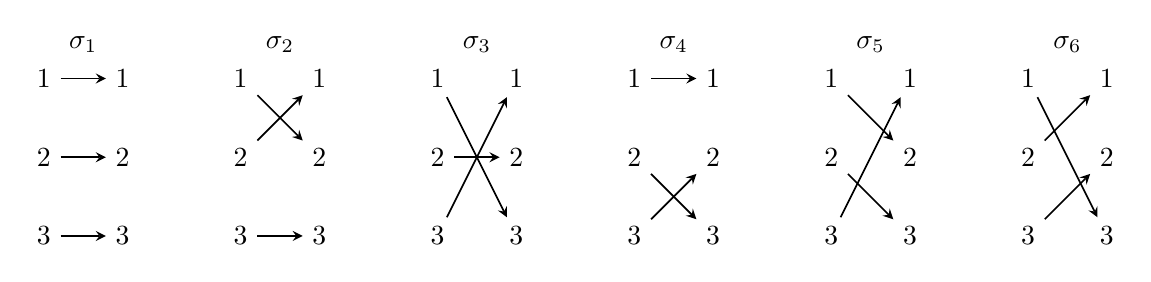
\begin{tikzpicture}
                \begin{scope}[xshift=0cm]
                    \node (1a) at (0,-1) {1};
                    \node (2a) at (0,-2) {2};
                    \node (3a) at (0,-3) {3};
                    \node (1b) at (1,-1) {1};
                    \node (2b) at (1,-2) {2};
                    \node (3b) at (1,-3) {3};
        
                    \node [above=2mm] at (0.5,-1) {$\sigma_1$};
        
                    \draw [semithick,-stealth] (1a) -- (1b);
                    \draw [semithick,-stealth] (2a) -- (2b);
                    \draw [semithick,-stealth] (3a) -- (3b);
                \end{scope}
                \begin{scope}[xshift=2.5cm]
                    \node (1a) at (0,-1) {1};
                    \node (2a) at (0,-2) {2};
                    \node (3a) at (0,-3) {3};
                    \node (1b) at (1,-1) {1};
                    \node (2b) at (1,-2) {2};
                    \node (3b) at (1,-3) {3};
        
                    \node [above=2mm] at (0.5,-1) {$\sigma_2$};
        
                    \draw [semithick,-stealth] (1a) -- (2b);
                    \draw [semithick,-stealth] (2a) -- (1b);
                    \draw [semithick,-stealth] (3a) -- (3b);
                \end{scope}
                \begin{scope}[xshift=5cm]
                    \node (1a) at (0,-1) {1};
                    \node (2a) at (0,-2) {2};
                    \node (3a) at (0,-3) {3};
                    \node (1b) at (1,-1) {1};
                    \node (2b) at (1,-2) {2};
                    \node (3b) at (1,-3) {3};
        
                    \node [above=2mm] at (0.5,-1) {$\sigma_3$};
        
                    \draw [semithick,-stealth] (1a) -- (3b);
                    \draw [semithick,-stealth] (2a) -- (2b);
                    \draw [semithick,-stealth] (3a) -- (1b);
                \end{scope}
                \begin{scope}[xshift=7.5cm]
                    \node (1a) at (0,-1) {1};
                    \node (2a) at (0,-2) {2};
                    \node (3a) at (0,-3) {3};
                    \node (1b) at (1,-1) {1};
                    \node (2b) at (1,-2) {2};
                    \node (3b) at (1,-3) {3};
        
                    \node [above=2mm] at (0.5,-1) {$\sigma_4$};
        
                    \draw [semithick,-stealth] (1a) -- (1b);
                    \draw [semithick,-stealth] (2a) -- (3b);
                    \draw [semithick,-stealth] (3a) -- (2b);
                \end{scope}
                \begin{scope}[xshift=10cm]
                    \node (1a) at (0,-1) {1};
                    \node (2a) at (0,-2) {2};
                    \node (3a) at (0,-3) {3};
                    \node (1b) at (1,-1) {1};
                    \node (2b) at (1,-2) {2};
                    \node (3b) at (1,-3) {3};
        
                    \node [above=2mm] at (0.5,-1) {$\sigma_5$};
        
                    \draw [semithick,-stealth] (1a) -- (2b);
                    \draw [semithick,-stealth] (2a) -- (3b);
                    \draw [semithick,-stealth] (3a) -- (1b);
                \end{scope}
                \begin{scope}[xshift=12.5cm]
                    \node (1a) at (0,-1) {1};
                    \node (2a) at (0,-2) {2};
                    \node (3a) at (0,-3) {3};
                    \node (1b) at (1,-1) {1};
                    \node (2b) at (1,-2) {2};
                    \node (3b) at (1,-3) {3};
        
                    \node [above=2mm] at (0.5,-1) {$\sigma_6$};
        
                    \draw [semithick,-stealth] (1a) -- (3b);
                    \draw [semithick,-stealth] (2a) -- (1b);
                    \draw [semithick,-stealth] (3a) -- (2b);
                \end{scope}
            \end{tikzpicture}
        \end{center}
        It follows that we may write
        \begin{align*}
            \sigma_1 &= \tau_{1,2}\tau_{1,2}&
            \sigma_2 &= \tau_{1,2}&
            \sigma_3 &= \tau_{1,3}&
            \sigma_4 &= \tau_{2,3}&
            \sigma_5 &= \tau_{1,2}\tau_{2,3}&
            \sigma_6 &= \tau_{1,2}\tau_{1,3}
        \end{align*}
    \end{proof}
    \setcounter{enumi}{8}
    \item Let $A:V\to W$ be a linear mapping. Show that if $T\in\alt[k]{W}$, then $A^*T\in\alt[k]{V}$.
    \begin{proof}
        % If $T\in\alt[k]{W}$, then $\Alt(\frac{1}{k!}T)=T$. Thus, $T^\sigma=\Alt(\frac{1}{k!}T)^\sigma=(-1)^\sigma\Alt(\frac{1}{k!}T)=(-1)^\sigma T$.

        % We have that $(A^*T)^\sigma=\Alt(\frac{1}{k!}A^*T)^\sigma


        Since $T\in\alt[k]{W}$, we know that $T^\sigma=(-1)^\sigma T$ for all $\sigma\in S_k$. It follows that
        \begin{align*}
            (A^*T)^\sigma(v_1,\dots,v_k) &= (A^*T)(v_{\sigma^{-1}(1)},\dots,v_{\sigma^{-1}(k)})\\
            &= T(Av_{\sigma^{-1}(1)},\dots,Av_{\sigma^{-1}(k)})\\
            &= T^\sigma(Av_1,\dots,Av_k)\\
            &= (-1)^\sigma T(Av_1,\dots,Av_k)\\
            &= (-1)^\sigma A^*T(v_1,\dots,v_k)
        \end{align*}
        as desired.
    \end{proof}
\end{enumerate}
\begin{enumerate}[label={\textbf{1.5.\roman*.}}]
    \item A $k$-tensor $T\in\lin[k]{V}$ is \textbf{symmetric} if $T^\sigma=T$ for all $\sigma\in S_k$. Show that the set $\sym[k]{V}$ of symmetric $k$-tensors is a vector subspace of $\lin[k]{V}$.
    \begin{proof}
        To prove that $\sym[k]{V}\leq\lin[k]{V}$, it will suffice to show that it contains the additive identity of $\lin[k]{V}$ (i.e., the zero tensor), and that it is closed under addition and scalar multiplication. Since we clearly have
        \begin{equation*}
            0^\sigma(v_1,\dots,v_k) = 0(v_{\sigma^{-1}(1)},\dots,v_{\sigma^{-1}(k)})
            = 0(v_1,\dots,v_k)
        \end{equation*}
        we know that $\sym[k]{V}$ contains the additive identity. Now suppose $T_1,T_2\in\sym[k]{V}$. Then since
        \begin{equation*}
            (T_1+T_2)^\sigma = T_1^\sigma+T_2^\sigma
            = T_1+T_2
        \end{equation*}
        where the first equality holds because of the linearity of $\sigma:\lin[k]{V}\to\lin[k]{V}$ and the second equality holds since $T_1,T_2\in\sym[k]{V}$, $\sym[k]{V}$ is closed under addition. Similarly, the fact that
        \begin{equation*}
            (\lambda T)^\sigma = \lambda T^\sigma
            = \lambda T
        \end{equation*}
        confirms that $\sym[k]{V}$ is closed under scalar multiplication.
    \end{proof}
\end{enumerate}
\begin{enumerate}[label={\textbf{1.6.\roman*.}}]
    \item Verify the following three equations, where $\lambda\in\R$.
    \begin{enumerate}
        \item $\lambda(\omega_1\wedge\omega_2)=(\lambda\omega_1)\wedge\omega_2=\omega_1\wedge(\lambda\omega_2)$.
        \begin{proof}
            We have that
            \begin{align*}
                \lambda(\omega_1\wedge\omega_2) &= \lambda\pi(T_1\otimes T_2)\\
                &= \pi[(\lambda T_1)\otimes T_2]\\
                &= (\lambda\omega_1)\wedge\omega_2
            \end{align*}
            It follows by a symmetric argument that $\lambda(\omega_1\wedge\omega_2)=\omega_1\wedge(\lambda\omega_2)$.
        \end{proof}
        \item $(\omega_1+\omega_2)\wedge\omega_3=\omega_1\wedge\omega_3+\omega_2\wedge\omega_3$.
        \begin{proof}
            We have that
            \begin{align*}
                (\omega_1+\omega_2)\wedge\omega_3 &= \pi[(T_1+T_2)\otimes T_3]\\
                &= \pi[T_1\otimes T_3+T_2\otimes T_3]\\
                &= \omega_1\wedge\omega_3+\omega_2\wedge\omega_3
            \end{align*}
            as desired.
        \end{proof}
        \item $\omega_1\wedge(\omega_2+\omega_3)=\omega_1\wedge\omega_2+\omega_1\wedge\omega_3$.
        \begin{proof}
            We have that
            \begin{align*}
                \omega_1\wedge(\omega_2+\omega_3) &= \pi[T_1\otimes(T_2+T_3)]\\
                &= \pi[T_1\otimes T_2+T_1\otimes T_3]\\
                &= \omega_1\wedge\omega_2+\omega_1\wedge\omega_3
            \end{align*}
            as desired.
        \end{proof}
    \end{enumerate}
    \item Verify the following multiplicative law for the wedge product.
    \begin{equation*}
        \omega_1\wedge\omega_2 = (-1)^{rs}\omega_2\wedge\omega_1
    \end{equation*}
    \begin{proof}
        As per \textcite{bib:DifferentialForms}, it suffices to prove this claim for decomposable elements. As such, let $\omega_1=\ell_1\wedge\cdots\wedge\ell_r$ and let $\omega_2=\ell_1'\wedge\cdots\wedge\ell_s'$. Let $\sigma\in S_{r+s}$ be the permutation
        \begin{equation*}
            \sigma(x) =
            \begin{cases}
                x+s & x\leq r\\
                x-r & x>r
            \end{cases}
        \end{equation*}
        We can write $\sigma$ as a product of elementary transpositions in a systematic manner as follows.
        \begin{equation*}
            \sigma = \prod_{j=s-1}^0\prod_{i=1}^r\tau_{i+j,\,i+j+1}
        \end{equation*}
        Clearly, there are $rs$ of these transpositions, so $(-1)^\sigma=(-1)^{rs}$. Therefore, we have that
        \begin{align*}
            \omega_1\wedge\omega_2 &= (\ell_1\wedge\cdots\wedge\ell_r)\wedge(\ell_1'\wedge\cdots\wedge\ell_s')\\
            &= (-1)^\sigma(\ell_1'\wedge\cdots\wedge\ell_s')\wedge(\ell_1\wedge\cdots\wedge\ell_r)\\
            &= (-1)^{rs}\omega_2\wedge\omega_1
        \end{align*}
    \end{proof}
    \stepcounter{enumi}
    \item If $\omega,\mu\in\lam[r]{V^*}$, prove that
    \begin{equation*}
        (\omega+\mu)^k = \sum_{\ell=0}^k\binom{k}{\ell}\omega^\ell\wedge\mu^{k-\ell}
    \end{equation*}
    (Hint: As in freshman calculus, prove this binomial theorem by induction using the identity $\binom{k}{\ell}=\binom{k-1}{\ell-1}+\binom{k-1}{\ell}$.)
    \begin{proof}
        We induct on $k$.\par
        For the base case $k=1$, we have that
        \begin{align*}
            \sum_{\ell=0}^1\binom{1}{\ell}\omega^\ell\wedge\mu^{1-\ell} &= \binom{1}{0}\omega^0\wedge\mu^{1-0}+\binom{1}{1}\omega^1\wedge\mu^{1-1}\\
            &= \mu+\omega\\
            &= (\omega+\mu)^1
        \end{align*}
        as desired.\par
        Now suppose inductively that we have proven the claim for $k-1$. Then
        \begin{align*}
            (\omega+\mu)^k &= (\omega+\mu)^1(\omega+\mu)^{k-1}\\
            &= (\omega+\mu)\sum_{\ell=0}^{k-1}\binom{k-1}{\ell}\omega^\ell\wedge\mu^{(k-1)-\ell}\\
            &= \sum_{\ell=0}^{k-1}\binom{k-1}{\ell}\omega^{\ell+1}\wedge\mu^{(k-1)-\ell}+\sum_{\ell=0}^{k-1}\binom{k-1}{\ell}\omega^\ell\wedge\mu^{k-\ell}\\
            &= \sum_{\ell=1}^k\binom{k-1}{\ell-1}\omega^{\ell}\wedge\mu^{k-\ell}+\sum_{\ell=0}^{k-1}\binom{k-1}{\ell}\omega^\ell\wedge\mu^{k-\ell}\\
            &= \binom{k-1}{k-1}\omega^{k-1}\wedge\mu^1+\sum_{\ell=1}^{k-1}\left[ \binom{k-1}{\ell-1}+\binom{k-1}{\ell} \right]\omega^{\ell}\wedge\mu^{k-\ell}+\binom{k-1}{0}\omega^0\wedge\mu^k\\
            &= \binom{k}{k}\omega^{k-1}\wedge\mu^1+\sum_{\ell=1}^{k-1}\binom{k}{\ell}\omega^{\ell}\wedge\mu^{k-\ell}+\binom{k}{0}\omega^0\wedge\mu^k\\
            &= \sum_{\ell=0}^k\binom{k}{\ell}\omega^{\ell}\wedge\mu^{k-\ell}
        \end{align*}
        as desired.
    \end{proof}
\end{enumerate}
\begin{enumerate}[label={\textbf{1.7.\roman*.}}]
    \item Prove that if $T$ is the decomposable $k$-tensor $\ell_1\otimes\cdots\otimes\ell_k$, then
    \begin{equation*}
        \iota_\vec{v}T = \sum_{r=1}^k(-1)^{r-1}\ell_r(\vec{v})\ell_1\otimes\cdots\otimes\hat{\ell}_r\otimes\cdots\otimes\ell_k
    \end{equation*}
    where the hat over $\ell_r$ means that $\ell_r$ is deleted from the tensor product.
    \begin{proof}
        We have that
        \begin{align*}
            (\iota_vT)(v_1,\dots,v_{k-1}) &= \sum_{r=1}^k(-1)^{r-1}T(v_1,\dots,v_{r-1},v,v_r,\dots,v_{k-1})\\
            &= \sum_{r=1}^k(-1)^{r-1}[\ell_1\otimes\cdots\otimes\ell_{r-1}\otimes\ell_r\otimes\ell_{r+1}\otimes\cdots\otimes\ell_k](v_1,\dots,v_{r-1},v,v_r,\dots,v_{k-1})\\
            &= \sum_{r=1}^k(-1)^{r-1}\ell_1(v_1)\cdots\ell_{r-1}(v_{r-1})\ell_r(v)\ell_{r+1}(v_r)\cdots\ell_k(v_{k-1})\\
            &= \sum_{r=1}^k(-1)^{r-1}\ell_r(v)\ell_1(v_1)\cdots\ell_{r-1}(v_{r-1})\ell_{r+1}(v_r)\cdots\ell_k(v_{k-1})\\
            &= \sum_{r=1}^k(-1)^{r-1}\ell_r(\vec{v})[\ell_1\otimes\cdots\otimes\hat{\ell}_r\otimes\cdots\otimes\ell_k](v_1,\dots,v_{k-1})
        \end{align*}
        as desired.
    \end{proof}
    \item Prove that if $T_1\in\lin[p]{V}$ and $T_2\in\lin[q]{V}$, then
    \begin{equation*}
        \iota_\vec{v}(T_1\otimes T_2) = \iota_\vec{v}T_1\otimes T_2+(-1)^pT_1\otimes\iota_\vec{v}T_2
    \end{equation*}
    \begin{proof}
        We have that
        \begin{align*}
            [\iota_\vec{v}(T_1\otimes T_2)](v_1,\dots,v_{p+q-1}) ={}& \sum_{r=1}^{p+q}(-1)^{r-1}(T_1\otimes T_2)(v_1,\dots,v_{r-1},v,v_r,\dots,v_{p+q-1})\\
            \begin{split}
                ={}& \sum_{r=1}^p(-1)^{r-1}(T_1\otimes T_2)(v_1,\dots,v_{r-1},v,v_r,\dots,v_{p+q-1})\\
                &+\sum_{r=p+1}^{p+q}(-1)^{r-1}(T_1\otimes T_2)(v_1,\dots,v_{r-1},v,v_r,\dots,v_{p+q-1})
            \end{split}\\
            \begin{split}
                ={}& \sum_{r=1}^p(-1)^{r-1}T_1(v_1,\dots,v_{r-1},v,v_r,\dots,v_{p-1})T_2(v_p,\dots,v_{p+q-1})\\
                &+\sum_{r=p+1}^{p+q}(-1)^{r-1}T_1(v_1,\dots,v_p)T_2(v_{p+1},\dots,v_{r-1},v,v_r,\dots,v_{p+q-1})
            \end{split}\\
            \begin{split}
                ={}& \left[ \sum_{r=1}^p(-1)^{r-1}T_1(v_1,\dots,v_{r-1},v,v_r,\dots,v_{p-1}) \right]\cdot T_2(v_p,\dots,v_{p+q-1})\\
                &+T_1(v_1,\dots,v_p)\cdot\sum_{r=p+1}^{p+q}(-1)^{r-1}T_2(v_{p+1},\dots,v_{r-1},v,v_r,\dots,v_{p+q-1})
            \end{split}\\
            \begin{split}
                ={}& \left[ \sum_{r=1}^p(-1)^{r-1}T_1(v_1,\dots,v_{r-1},v,v_r,\dots,v_{p-1}) \right]\cdot T_2(v_p,\dots,v_{p+q-1})\\
                &+T_1(v_1,\dots,v_p)\cdot(-1)^p\sum_{r=1}^q(-1)^{r-1}T_2(v_{p+1},\dots,v_{p+r-1},v,v_{p+r},\dots,v_{p+q-1})
            \end{split}\\
            \begin{split}
                ={}& (\iota_vT_1)(v_1,\dots,v_{p-1})\cdot T_2(v_p,\dots,v_{p+q-1})\\
                &+(-1)^pT_1(v_1,\dots,v_p)\cdot(\iota_vT_2)(v_{p+1},\dots,v_{p+q-1})
            \end{split}\\
            ={}& (\iota_vT_1\otimes T_2)(v_1,\dots,v_{p+q-1})+(-1)^p(T_1\otimes\iota_vT_2)(v_1,\dots,v_{p+q-1})\\
            ={}& [\iota_\vec{v}T_1\otimes T_2+(-1)^pT_1\otimes\iota_\vec{v}T_2](v_1,\dots,v_{p+q-1})
        \end{align*}
        as desired.
    \end{proof}
    \item Show that if $T\in\alt[k]{V}$, then $\iota_\vec{v}T=kT_\vec{v}$, where $T_\vec{v}$ is defined as in Exercise 1.3.vii. In particular, conclude that $\iota_\vec{v}T\in\alt[k-1]{V}$. (See Exercise 1.4.viii, which asserts that $T\in\alt[k]{V}$ implies $T_\vec{v}\in\alt[k-1]{V}$.)
    \begin{proof}
        Suppose $T\in\alt[k]{V}$. Let $\sigma\in S_k$ be the permutation that moves the $r^\text{th}$ index to the first place and shifts all $r-1$ indices to its left up one. For example, if $r=4$ and $\sigma\in S_6$, $\sigma(1,2,3,4,5,6)=(4,1,2,3,5,6)$. More relevant to our situation would be the ability of $\sigma$ to do the following.
        \begin{equation*}
            \sigma(v_1,v_2,v_3,v,v_4,v_5) = \sigma(v,v_1,v_2,v_3,v_4,v_5)
        \end{equation*}
        Going back to the general case, since we have
        \begin{equation*}
            \sigma = \prod_{i=1}^{r-1}\tau_{i,i+1}
        \end{equation*}
        we can determine that
        \begin{equation*}
            (-1)^\sigma = (-1)^{r-1}
        \end{equation*}
        Therefore, by the above and since $T^\sigma=(-1)^\sigma T$ as an alternating $k$-tensor,
        \begin{align*}
            (\iota_vT)(v_1,\dots,v_{k-1}) &= \sum_{r=1}^k(-1)^{r-1}T(v_1,\dots,v_{r-1},v,v_r,\dots,v_{k-1})\\
            &= \sum_{r=1}^k(-1)^\sigma T(v_1,\dots,v_{r-1},v,v_r,\dots,v_{k-1})\\
            &= \sum_{r=1}^kT^\sigma(v_1,\dots,v_{r-1},v,v_r,\dots,v_{k-1})\\
            &= \sum_{r=1}^kT(v,v_1,\dots,v_{k-1})\\
            &= \sum_{r=1}^kT_v(v_1,\dots,v_{k-1})\\
            &= kT_v(v_1,\dots,v_{k-1})
        \end{align*}
        as desired.\par
        As stated in the question, we may invoke Exercise 1.4.vii to determine that $\iota_vT=kT_v\in\alt[k-1]{V}$.
    \end{proof}
\end{enumerate}
\begin{enumerate}[label={\textbf{1.8.\roman*.}}]
    \item Verify the following assertions.
    \begin{enumerate}
        \item The map $A^*:\lam[k]{W^*}\to\lam[k]{V^*}$ sending $\omega\mapsto A^*\omega$ is linear.
        \begin{proof}
            We have that
            \begin{align*}
                A^*(\omega_1+\omega_2) &= \pi(A^*(T_1+T_2))&
                    A^*(\lambda\omega) &= \pi(A^*(\lambda T))\\
                &= \pi(A^*T_1+A^*T_2)&
                    &= \pi(\lambda A^*T)\\
                &= \pi(A^*T_1)+\pi(A^*T_2)&
                    &= \lambda\pi(A^*T)\\
                &= A^*\omega_1+A^*\omega_2&
                    &= \lambda A^*\omega
            \end{align*}
            as desired.
        \end{proof}
        \item If $\omega_i\in\lam[k_i]{W^*}$ ($i=1,2$), then
        \begin{equation*}
            A^*(\omega_1\wedge\omega_2) = A^*(\omega_1)\wedge A^*(\omega_2)
        \end{equation*}
        \begin{proof}
            We have that
            \begin{align*}
                A^*(\omega_1\wedge\omega_2) &= A^*(\pi(T_1\otimes T_2))\\
                &= \pi(A^*(T_1\otimes T_2))\\
                &= \pi(A^*T_1\otimes A^*T_2)\\
                &= \pi(A^*T_1)\wedge\pi(A^*T_2)\\
                &= A^*(\omega_1)\wedge A^*(\omega_2)
            \end{align*}
            as desired.
        \end{proof}
        \item If $U$ is a vector space and $B:U\to V$ is a linear map, then for $\omega\in\lam[k]{W^*}$,
        \begin{equation*}
            B^*A^*\omega = (AB)^*\omega
        \end{equation*}
        \begin{proof}
            We have that
            \begin{align*}
                B^*A^*\omega &= B^*(\pi(A^*T))\\
                &= \pi(B^*A^*T)\\
                &= \pi((AB)^*T)\\
                &= (AB^*)\omega
            \end{align*}
            as desired.
        \end{proof}
    \end{enumerate}
    \item Deduce from the fact "$A:V\to V$ not surjective implies $\det(A)=0$" a well-known fact about determinants of $n\times n$ matrices: If two columns are equal, the determinant is zero.
    \begin{proof}
        If an $n\times n$ matrix has two identical columns, then the dimension of its range space is at most $n-1$. Thus, $A$ is not surjective, and hence has $\det(A)=0$.
    \end{proof}
    \stepcounter{enumi}
    \item Deduce from Exercise 1.8.i another well-known fact about determinants of $n\times n$ matrices: If $(b_{i,j})$ is the inverse of $[a_{i,j}]$, its determinant is the inverse of the determinant of $[a_{i,j}]$.
    \begin{proof}
        Let $(b_{i,j})=[a_{i,j}]^{-1}$. Then
        \begin{equation*}
            (b_{i,j})[a_{i,j}] = \id_V
        \end{equation*}
        It follows from Propositions 1.8.7 and 1.8.8 (which in turn follow from Exercise 1.8.i) that
        \begin{align*}
            \det(b_{i,j})\det[a_{i,j}] &= \det(\id_V) = 1\\
            \det(b_{i,j}) &= \frac{1}{\det[a_{i,j}]}
        \end{align*}
        as desired.
    \end{proof}
    \item Extract from the formula $\det([a_{i,j}])=\sum_{\sigma\in S_n}(-1)^\sigma a_{1,\sigma(1)}\cdots a_{n,\sigma(n)}$ the following well-known formula for determinants of $2\times 2$ matrices.
    \begin{equation*}
        \det
        \begin{pmatrix}
            a_{11} & a_{12}\\
            a_{21} & a_{22}\\
        \end{pmatrix}
        = a_{11}a_{22}-a_{12}a_{21}
    \end{equation*}
    \begin{proof}
        The two elements of $S_2$ are the identity permutation (which we will refer to as $\sigma_1$) and $\tau_{1,2}$ (which we will refer to as $\sigma_2$). It follows that for the $n=2$ case,
        \begin{align*}
            \det
            \begin{pmatrix}
                a_{11} & a_{12}\\
                a_{21} & a_{22}\\
            \end{pmatrix}
            &= \sum_{\sigma\in S_2}(-1)^\sigma a_{1,\sigma(1)}a_{2,\sigma(2)}\\
            &= (-1)^{\sigma_1}a_{1,\sigma_1(1)}a_{2,\sigma_1(2)}+(-1)^{\sigma_2}a_{1,\sigma_2(1)}a_{2,\sigma_2(2)}\\
            &= (1)a_{1,1}a_{2,2}+(-1)a_{1,2}a_{2,1}\\
            &= a_{1,1}a_{2,2}-a_{1,2}a_{2,1}
        \end{align*}
        as desired.
    \end{proof}
\end{enumerate}
\begin{enumerate}[label={\textbf{1.9.\roman*.}}]
    \item Prove that if $\vec{e}_1,\dots,\vec{e}_n$ is a positively oriented basis of $V$, then the basis $\vec{e}_1,\dots,\vec{e}_{i-1},-\vec{e}_i,\vec{e}_{i+1},\dots,\vec{e}_n$ is negatively oriented.
    \begin{proof}
        Since $\vec{e}_1,\dots,\vec{e}_n$ is a positively oriented basis of $V$, we know that $e_1^*\wedge\cdots\wedge e_n^*\in\lam[n]{V^*}_+$. This combined with the fact that
        \begin{equation*}
            \vec{e}_1\wedge\cdots\wedge\vec{e}_{i-1},-\vec{e}_i,\vec{e}_{i+1}\wedge\cdots\wedge\vec{e}_n = -e_1^*\wedge\cdots\wedge e_n^*
            \notin \lam[n]{V^*}
        \end{equation*}
        implies that the given basis is negatively oriented, as desired.
    \end{proof}
    \item Show that the argument in the proof of Theorem 1.9.9 can be modified to prove that if $V$ and $W$ are oriented, then these orientations induce a natural orientation on $V/W$.
    \begin{proof}
        Let $W\leq V$, $\dim V=n>1$, $\dim W=k<n$, and $r=n-k$. WLOG choose $e_1,\dots,e_n$ a positively oriented basis of $V$ such that $e_{r+1},\dots,e_n$ is a positively oriented basis of $W$. It follows that $\pi(e_1),\dots,\pi(e_r)$ for a basis of $V/W$. Assign to $V/W$ the orientation associated with this basis.\par
        Now suppose $\pi(f_1),\dots,\pi(f_r)$ is another basis of $V/W$.
    \end{proof}
\end{enumerate}




\end{document}